\documentclass[11pt,letterpaper]{article}

\usepackage{natbib}
%\usepackage{cite}
\usepackage{graphicx}
\usepackage[margin=1.in,centering]{geometry}
\usepackage{hyperref}


\begin{document}

\title{Optical/UV Band
Reverberation Mapping of NGC 5548 with Frequency-Resolved Techniques}

\author{Otho A. Ulrich,$^{1,2}$ Edward M. Cackett$^{1}$
\\
% List of institutions
$^{1}$Department of Physics and Astronomy, Wayne State University\\
$^{2}$Department of Physics, Western Michigan University\\
}
\date{August 8, 2016}

\maketitle

\begin{abstract}

Power spectral densities and time delays of 19 wavelength bands are recovered as part of a reverberation mapping of NGC 5548. The latest time-variable light curves are made available in STORM III by \cite{2016ApJ...821...56F}. The uneven distribution of flux data in those curves necessitates the use of a maximum likelihood method in conjunction with Fourier transformations to produce the frequency-dependent values of interest. Variability in the emissions is confirmed in the power spectral densities, and the time delays show the expected frequency dependence. The time delays also appear to have wavelength dependence. There are issues computing accurate error estimates for both distributions that remain as yet unresolved. The transfer function should be recoverable once those and any additional computational issues are resolved.

\end{abstract}

\section{Introduction}

The local Type-I Seyfert galaxy NGC 5548, while perhaps the best-studied active galaxy, remains an object of intense interest and study to modern astronomy. Direct observation of active galactic nuclei (AGN) such as that thought to exist at the center of NGC 5548 is rarely possible. The astronomer may infer the properties of AGN from the dynamics of their variable spectra. \cite{2016ApJ...821...56F} published the most complete set of time-dependent light curves yet collected from an active galactic nucleus as part III of STORM, an extensive optical/UV observational campaign carried out on NGC 5548. We now attempt to use frequency-domain analyses to map the reverberation in the observed light curves.

\section{Reverberation Mapping}
	One model for AGN suggests that a hot accretion disk is incident upon a central super-massive black hole (SMBH). Electromagnetic emission emergent from the gas surrounding the SMBH is reprocessed by the disk, resulting in observed response delays between emission peaks. If the temperature of the disk decreases radially from the SMBH, the observed time delays can be expected to increase with decreasing wavelength. A transfer function encodes the geometry of the system by describing the time-dependent response of each light curve against the others. Recovering the function from the observed light curves is a primary goal of reverberation mapping.

	This technique has become a standard for calculating the black hole mass of AGN. It is well-described by \cite{2007MNRAS.380..669C} and \cite{2014A&ARv..22...72U} and many others. It continues to be refined, and may also become a tool to measure the black hole spin of these systems (\cite{2016arXiv160606736K}).

	\begin{figure}
		\centering
		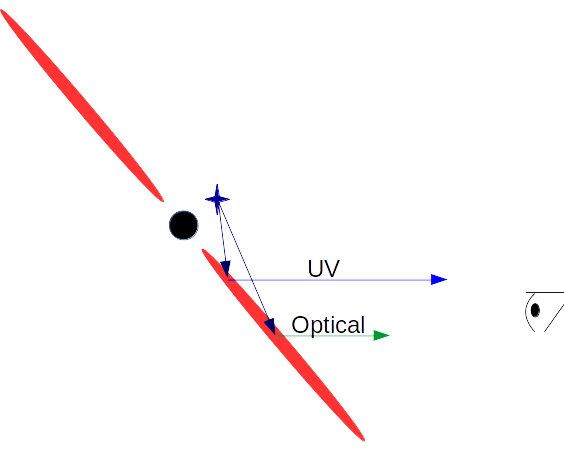
\includegraphics[width=3.5in]{../img/basic_geometry.png}
		\caption{Simple geometry of reverberation in the accretion disk. Some continuum emissions are reprocessed before escaping toward the observer.}
	\end{figure}

\subsection{Frequency-domain Analysis}

	The transfer function is related to two light curves as being convoluted against the reference light curve (\ref{time_transfunc}). The convolution theorem 

	\begin{equation}
		\label{time_transfunc}
		y(t) = \int_{-\infty}^{\infty} g(\tau) x(t-\tau)  {\rm d}\tau
	\end{equation}

	\begin{equation}
		\label{freq_transfunc}
		Y(\nu) = G(\nu) X(\nu)
	\end{equation}



	The power spectral density (PSD) for a given emission band can be produced using Fourier transforms, providing a measure of the time-scale of variability in that band. Given two bands, typically a reference or "driving" band and a delayed or "response" band, a cross spectrum can also be constructed. From the complex argument of the cross-correlation function, one can derive the frequency-dependent time delay between those bands; an important step toward constituting the transfer function of a system. Very good explanations of these techniques and the associated mathematics are available from \cite{2014A&ARv..22...72U}.

	A top-hat function provides a simple model of the impulse response of a delayed light curve. A fast Fourier transform method of this impulse response provides the time delay spectrum as a function of temporal frequency. This simple model provides a guideline for how the computed time delays are expected to be distributed as a function of temporal frequency.

	(Side-by-side graphic of top-hat impulse response function and FFT of top-hat giving time delays.)

	\subsection{Unevenly-Sampled Data}


	Optical reverberation mapping techniques involve time-domain analyses, such as cross-correlation. Time-domain techniques have limitations: cross-correlation, for instance, provides only the average time delay between two light curves; they also require data that is evenly-sampled across the time domain. X-ray reverberation mapping in particular has developed a body of techniques based on frequency-domain techniques, primarily Fourier analysis; these techniques still require evenly-sampled data and have been enabled by the relatively good data coverage in X-ray bands. They provide the astronomer with more detailed information about the variability and response delay within the system compared to time-domain techniques.


 	Some X-ray datasets contain gaps due to orbital mechanics, which motivated the work in \cite{2013ApJ...777...24Z}, where a maximum likelihood method is used to perform Fourier analysis on light curves with gaps. Since its development, this technique has found success among studies of observations captured by low-orbit X-ray telescopes that exceed the telescopes' orbital periods, such as the analysis performed by \cite{2016arXiv160606736K}. Until now, reverberation mapping in the optical bands has been limited to time-domain techniques. Many datasets available for these bands have uneven sampling across the time domain, however, and so do not lend themselves well to time-domain or traditional frequency-domain analyses. The maximum likelihood method is well-suited to extracting useful information from the data available in those datasets.

\section{Analysis}
The 1367\AA$ $ light curve, obtained from observations made with the Hubble Space Telescope, is chosen as the reference curve. The power spectral densities and time delays as a function of temporal frequency are computed for each band in the dataset -- 18 bands not including the reference band.

The light curves analysed here are unevenly distributed along the time axis, which suggests that the maximum likelihood method developed by \cite{2013ApJ...777...24Z} is a reasonable candidate for producing the PSD and time delays in the frequency domain. The latest version (CHECK THIS) of the C++ program psdlag associated with that work is used to directly produce the PSD and cross spectra. The time delay spectrum is produced from the cross spectrum by dividing it by $2 \pi f$, with $f$ the mean frequency for a given bin.

	\subsection{Dataset}
	\cite{2016ApJ...821...56F} published the best dynamic data yet collected from NGC 5548 over a 200-day (CHECK THIS) period, for 19 bands throughout the optical and into the UV spectra. These data were collected from a variety of observatories, including both space and ground-based telescopes, and thus have significantly variable sampling rates.

	(Include picture of Fausnaugh data here)

	\subsection{Error Analysis}
	For the presented set of resultant data, the error estimates are extracted from the covariance matrix. This method assumes that the errors between frequency bins are not correlated, so these values only represent a lower limit of the true variability. Scanning the likelihood function can provide better error estimates at the cost of computation time, as can running Monte Carlo simulations. All of these methods are built into the psdlag program provided by \cite{2013ApJ...777...24Z}, however, some issues have prevented proper error analysis using the latter two methods. This is discussed in more detail in section \ref{results}.

\section{Results}
\label{results}

An atlas of the power spectral densities as functions of temporal frequency for all 18 delayed bands is provided in this section. One is also provided of the time delay spectra for each band. The reference band PSD is also provided separately. Errors presented in these atlases are obtained from the covariance matrix.

(Atlas of PSD)

(Atlas of Time Delays)

	\subsection{Dubious Error Computations}
	The errors obtained from the covariance matrix are only a lower estimate of the true error. An error analysis by scanning the likelihood function was attempted, but dubious values led to their exclusion from these results. In the case of

	(Example of bad LF error)

	Monte Carlo simulations were also attempted as a way of estimating the variability of the resultant values. Many errors obtained from this method were much larger than the expected accurate values. Therefore, this analysis was also excluded.

	(Example of bad MC error)


\section{Discussion}
Frequency-dependent power spectral densities confirm time-dependent variability in the emission strengths for each band. This behaviour is expected for any active galactic nucleus and has been long-confirmed in NGC 5548, so it comes as no surprise to find those results here.

Analysis of the top-hat impulse response model predicted frequency-dependent time delays, which have been recovered from the light curves in this analysis. Furthermore, the distribution of time delays indicates a wavelength-dependent nature. This warrants further study and analysis.

(Maybe a graph comparing the top-hat time delays to one band's time delays.)

The analyses performed on these data have elucidated clear trends in the PSD and time delays. With reverberation mapping, the goal is to recover the transfer function, which encodes the geometry of the system. Recovering the time delays is a significant step toward that goal.

%\bsp
\bibliographystyle{plainnat}
\bibliography{wsu_reu}





Consider two lightcurves $x(t)$ and $y(t)$, where $x(t)$ is the driving lightcurve and $y(t)$ is the reprocessed lightcurve.  If they are related by a linear impulse response, $g(\tau)$, then: 









So, $y(t)$ is a delayed and blurred version of $x(t)$, with the amount of delay and blurring encoded in $g(\tau)$.

The power spectral density (PSD) of $x(t)$ is calculated from the Fourier transform of $x(t)$, which we denote $X(\nu)$.  The PSD is $|X(\nu)|^2 = X^*(\nu)X(\nu)$, where the $^*$ denotes the complex conjugate.  From the convolution theorem of Fourier transforms we can write:



This means it is easy to relate the PSD of the reprocessed lightcurve to the PSD of the driving lightcurve and the impulse response function:

\begin{equation}
|Y(\nu)|^2 = |G(\nu)|^2 |X(\nu)|^2
\end{equation}

The cross spectrum is defined as
\begin{equation}
C(\nu) = X^*(\nu) Y(\nu)
\end{equation}
the phase, $\phi$, of which gives the phase lag between X and Y at each Fourier frequency, $\nu$.  This can be converted to a time lag through: 
\begin{equation}
\tau(\nu) = \frac{\phi(\nu)}{2\pi\nu}
\end{equation}
Since $Y(\nu) = G(\nu) X(\nu)$,  the cross spectrum can be written as:
\begin{equation}
C(\nu) = X^*(\nu) G(\nu) X(\nu) =  G(\nu) |X(\nu)|^2 
\end{equation}
thus, for a given impulse response function, one can trivially predict the time lags as a function of frequency, $\tau(\nu)$, by calculating the phase of $G(\nu)$, and the frequency dependence of the lags directly relates to the shape of the response function.







\end{document}